\documentclass[11pt,a5paper]{book}
\usepackage[utf8]{inputenc}
\usepackage{amsmath}
\usepackage{amsfonts}
\usepackage{amssymb}
\usepackage{graphicx}
\usepackage[super]{nth}
\usepackage{float}

\title{One Fish, Two Fish}
\author{Marcel Gietzmann-Sanders}
\date{}
\setcounter{tocdepth}{1}
\begin{document}
\maketitle
\tableofcontents
\newpage
\chapter{How to Digest a Brick}

\section{Well What's the Point?}

Quantitative fisheries science (hereafter referred to just as fisheries modeling) is all about the following question:
\newline

\hangafter=0 \hangindent=1cm \noindent How can a fishery bring the most long term benefit to society?
\newline

Nice and clear, right? Hardly. This is one of those wonderfully simplistic statements that throws a veil of apparent clarity over an entangled mass of delicious complexity. In other words, there's a lot to unpack.
\newline

Like all such statements all it takes is the most rudimentary of questions to blow its cover. For example - what is a fishery? That's a question biologists are still arguing about and we've been fishing in all likelihood since before the dawn of fire itself! 
\newline

Fortunately humans are pretty good at pretending the world is a lot simpler than it is and somehow managing to get away with it. So the fact that we've been able to declare dozens of "Sexiest People Alive" but are still ruminating on what a fishery is hasn't prevented us from making some good progress in the matter of getting fish on a plate. 
\newline

That being said the fun in a question like this one is not in just saying it. No, as anyone who watches true crime knows - the verdict only matters because of the story that unravels around it. 
So let's do some unraveling shall we? 
\newpage

\noindent \rule{\textwidth}{0.5pt} 
\noindent How can a \textbf{fishery} bring the most long term benefit to society?
\newline
\rule{\textwidth}{0.5pt} 
\vspace{5pt}

I know what you're thinking. Didn't I just say that no one's actually been able to agree on \textit{exactly} what a fishery is? So how on earth do I suppose I'm about to answer the question myself? Well that's one of the privileges that comes with being the one who writes this story.
\newline

In all seriousness though, if I don't at least present a working definition... well then we'll have nothing to work with and we'll just end up missing each other like two ships in the dark for the rest of this book. So consider this definition not so much an audacious claim on my part and more as a desperate attempt to try find some common ground for us to stand on for whatever time you'll give me. 
\newline

Alright, here goes. A fishery in this book is going to mean a specific group of marine populations, at least one of which we catch and use. This definition is nice because it allows for ecosystem based management where we consider the interactions between species while also allowing us to talk about the more tradition forms of management that work with one species at a time. 
\newline

That being said it's worth noting that I'm looking at the population as a whole. And that means I'm roping in \textit{everyone} who touches it. Unintended catch (bycatch), intended catch, commercial, recreational, artisinal, I'm throwing the all in the same... well... boat. I think as we continue to pull the thread and unravel this problem it will become clear why I've decided to do this, but just be warned that often times a fishery means the opposite of what I've defined and rather than focusing on the population it focuses on the human groupings fishing it. 
\newpage

\noindent \rule{\textwidth}{0.5pt} 
\noindent How can a fishery bring the most long term \textbf{benefit} to society?
\newline
\rule{\textwidth}{0.5pt} 
\vspace{5pt}

If defining a fishery was difficult, defining what benefit to society means is even more so. Which is why I'm just not going to bother.
\newline

At least not now.
\newline

Benefits to society are marvelously specific to the fishery in question and for that matter to the society in question as well. Benefits from seafood can be nutritional, cultural, financial, ecological, spiritual... yea you get the idea. Fisheries can make or break communities, they provide medical inputs, represent a multi-billion dollar industry, provide a primary source of protein to a good half of the entire world population, and are, quite critically, an essential part of an unnerving proportion of my lunches (although I may be a bit biased on that last point).
\newline

My point is simple - benefits cannot be defined in the abstract, you have to get down and dirty to \textit{really} understand what a fishery does and \textit{can} mean to society. 
\newline

\textit{Know thy fishery}.
\newpage


\noindent \rule{\textwidth}{0.5pt} 
\noindent How can a fishery bring the most \textbf{long term} benefit to society?
\newline
\rule{\textwidth}{0.5pt} 
\vspace{5pt}

We live in the post-modern world. If you don't know what sustainability means or why it's important it's time to start thinking about renting. I hear living under a rock isn't good for your health.
\newline

If on the other hand you happen to be someone just looking for a deeper sense of what sustainability means, then read on! There's definitely a lot to unpack on how to evaluate the sustainability of a natural resource.
\newpage


\noindent \rule{\textwidth}{0.5pt} 
\noindent How can a fishery bring the \textbf{most} long term benefit to society?
\newline
\rule{\textwidth}{0.5pt} 
\vspace{5pt}

This now, well this is the question that brings out the pitchforks, firebrands, and lobbyists. It's one thing to acknowledge all the benefits a fishery can bring to society - figuring out how to balance all of these value propositions is quite another thing. Behind struggling with the question of who society is and how to make sure it is represented, this balancing act may be the single most important activity in fisheries management which is exactly why I'm not going to attempt to answer the question at all. 
\newline

I am not judge, jury, and executioner - I'm just a dude who likes fish, numbers, and environmental stewardship. But suffice it to say, fisheries scientists have a \textit{responsibility} to help ensure that political conversation is as data driven as possible and then when possible win-win situations are discovered even if the interested parties are more interested in fighting for their stake in it all.
\newline

Just as importantly it's paramount that every fisheries scientist out there recognizes that while their science may seem impartial or whatever there is always an implicit balance of benefits in every single optimization we ever do. That's a hard truth one can never escape. No what you're fighting for, because any and all data represents ammunition for someone. 
\newpage

\noindent \rule{\textwidth}{0.5pt} 
\noindent \textbf{How} can a fishery bring the most long term benefit to society?
\newline
\rule{\textwidth}{0.5pt} 
\vspace{5pt}

Obviously there are loads of ways to improve the benefits to society. Finding better ways to fish, setting catch limits to prevent the merciless decimation of a fish stock, being smarter about what's taken and what's left to pull in the most valuable fish - these are some of the more apparent ones. However there are loads of other ways - becoming a restaurateur who changes the public opinion about a specific species of fish, developing monitoring for the supply chain to help people understand where their food is coming from, there are a lot of really cool and interesting options. 
\newline

However I know I've got limited time with you and so for the sake of brevity (and some fantastic novels probably sitting on your shelf right now) I'm going to have to limit scope. So we're going to focus on being creative about the actions the fishers themselves can take when out actually catching the fish. 
\newpage

\noindent \rule{\textwidth}{0.5pt} 
\noindent  How can a fishery bring the maximum long term benefits to \textbf{society}?
\newline
\rule{\textwidth}{0.5pt} 
\vspace{5pt}

This is a question with an obvious answer that probably should be paid more attention to. Society is \textit{all} of us. It's not just mega-corps, it's not just the town near the fish that's been fishing there for centuries, and its not the consumer either. It is \textit{everyone} and making sure \textit{all} are represented is of utmost importance. 
\newline

And as with the "most" question each and every model we build, each optimization we run, has implicit notions about \textit{who} society is. Be conscientious of that. 
\newpage

Alright, with all of that in mind I think our question is looking a little bit different. 
\newline

\hangafter=0 \hangindent=1cm \noindent \textbf{Fisheries modeling is about informing the set of fishing practices that would maximize a specific balance of benefits in a sustainable fashion. This information should then be used as part of a representative collaboration to find the balance best suited to the whole.}
\newline

So what's needed to make this happen? By a wonderful coincidence that just happens to be what the next section is about. 
\newpage

\section{The 30,000 Foot View}

\noindent \rule{\textwidth}{0.5pt} 
\begin{figure}[h!] 
  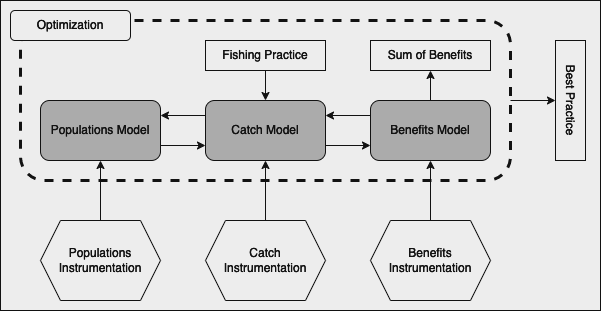
\includegraphics[width=\linewidth]{drawings/high_level_models.png}
  \caption{Models}
  \label{fig:high_level_models}
\end{figure}
\newline
\rule{\textwidth}{0.5pt} 
\vspace{5pt}

The first thing we need is a series of models that will allow us to... well... model how changing fishing practice will effect our overall benefit. These models divide into, broadly speak, three different categories. 
\newline

The benefits model is how we derive, from a specific situation, what the expected long term benefit would be. For example if the \textit{only} benefit is economic first sale benefit based on weight then the relationship between weight and cost would be one aspect of our model. This could then be applied to the expected catch each year (structured by weight of course) to then produce an expected value of the fishery year over year which could then be integrated to give us the long term benefit. In general however benefits models are far more complicated than this as, as we've already mentioned, there's a lot more to benefit that just value per weight class.
\newline

The second model we need is the population model. This describes how the populations in question change in response to the environment around them (which can include the fishers). A simple example would be a model that predicts the amount of recruitment (new fish babies) to the population as a function of the current population along with a model of how quickly the fish die off from natural mortality as the years go by. These two then allow us to predict how the population will change over time. However these models can get far more complex than just this (and most often do). 
\newline

In the middle of these two models we need a catch model. This is the model that describes how our choices in managing the fishery effect the underlying populations. Often times this model is as simple as a relationship between fishing effort and fishing mortality with some notion of gear selectivity included (gear selectivity being the fact that a specific kind of gear will typically catch a particular kind of age or weight of fish). Without this model there's no way to connect our benefit model to the population model. It's also the model that takes the parameters of fishery action that we're ultimately using as the knobs to tune to optimize our overall sustained benefit to society. 
\newpage

\noindent \rule{\textwidth}{0.5pt} 
\begin{figure}[h!] 
  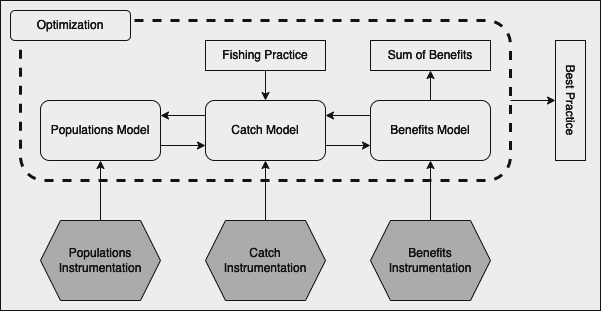
\includegraphics[width=\linewidth]{drawings/high_level_instrumentation.png}
  \caption{Instrumentation}
  \label{fig:high_level_instrumentation}
\end{figure}
\newline
\rule{\textwidth}{0.5pt} 
\vspace{5pt}

We've been talking about models quite flippantly so far. But all models are approximations of reality that need to be fit. What does fitting mean? Let's take a look at a simple example. One thing that fisheries scientists often have to model is the relationship between age (usually in years $t$) to body length $L$. One such model is the Von Bertalanffy growth curve:

$$L = L_{\infty}(1-e^{-Kt})$$


As with all models, this model divides into three parts: input variables - $t$, output variables - $L$, and parameters - $L_{\infty}$ and $K$. The input variables are things we'd measure and the output variables are what we want to predict but in order to do so we need to choose specific values for the parameters. Well you'd start with measurements like in Fig. \ref{fig:length_measurements_by_year}.


\begin{figure}[H] 
  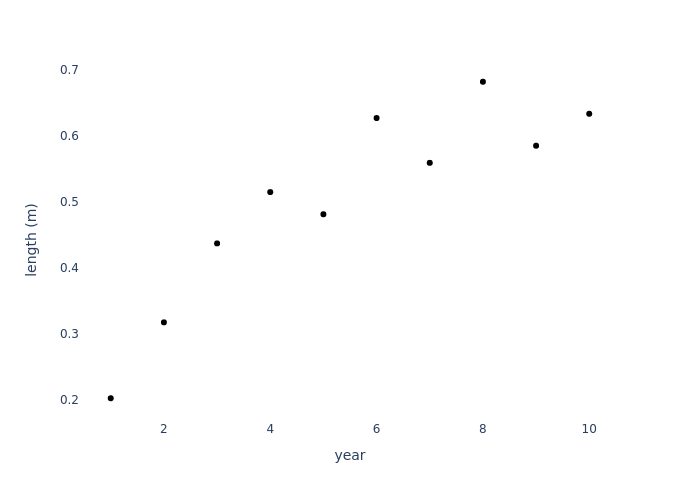
\includegraphics[scale=0.35]{notebooks/Fitting/new_measurements.png}
  \caption{Average Length Measurements by Year}
  \label{fig:length_measurements_by_year}
\end{figure}

Now the question is how do we find the parameters that best "fit" this data? Well from our equation we know that eventually (as $t \rightarrow \infty$) our length will go to $L_\infty$. So looking at this data we can guess that $L_\infty = 0.7$.  
\newline

However, what value should we assign to $K$? Well what we can do is try several values and see which fits best.

\begin{figure}[H] 
  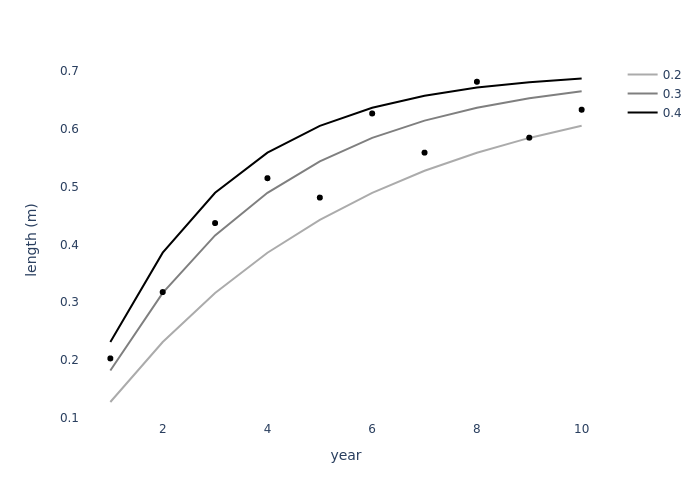
\includegraphics[width=\linewidth]{notebooks/Fitting/fit_lines.png}
  \caption{Attempting to Fit $K$}
  \label{fig:fitting_K}
\end{figure}

Fig. \ref{fig:fitting_K} shows us the predicted length vs year relationship for three values of $K$, 0.2, 0.3, and 0.4. By just visual inspection we can see that 0.2 doesn't grow fast enough whereas 0.4 grows to quickly, so 0.3 is probably a reasonable fit.
\newline

In general there are automated mechanisms for doing this but the lesson remains the same - to fit a model you need measurements that can act as ground truth for your fitting (or training) procedure. And that means that for each and every one of our models we're going to need instrumentation to generate that ground truth data. 
\newpage

\noindent \rule{\textwidth}{0.5pt} 
\begin{figure}[h!] 
  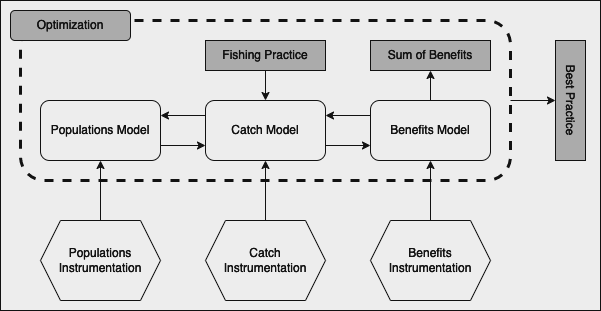
\includegraphics[width=\linewidth]{drawings/high_level_optimization.png}
  \caption{Optimization}
  \label{fig:high_level_optimization}
\end{figure}
\newline
\rule{\textwidth}{0.5pt} 
\vspace{5pt}

Alright so we've got ourselves some models that have been fit using the data from the corresponding instrumentation. Now what? Well now we're in a position to use these models to determine what the best fishing practice looks like. Let's take a real simple example to illustrate this.
\newline

All optimizations begin with clearly parametrizing the boundaries of the management practice. In our case, to keep things simple, we're going to assume that we're just directly controlling fishing mortality $F$. Now the basic population model we'll use will assume that if $Z$ is the overall instantaneous mortality rate for fish, in other words we have:

$$\frac{dN}{dt}=-ZN$$

which more or less reads as - we loose population at a rate of $Z\%$ of the overall population size. This is a pretty standard exponential growth equation whose solution is:

$$N = N_0 e^{-Zt}$$

Next we'll also assume we're in an equilibrium state such that the development of one age group describes the whole population. Therefore in year $t_y$ the population size:

$$N_y = N_0 e^{-Zt_y}$$

Next we're going to make the assumption that our $Z=M+F$ where $M$ is the natural mortality (fit with our instrumentation data). 
\newline

This gives our population model. How about the catch model? Well we know that $F/Z$ represents the portion of the mortality that ends up as catch. So if the overall fish mortality in an age class $D_y$ is given by:

$$D_y = N_{y-1} - N_y =N_0(e^{-Zt_{y-1}}- e^{-Zt_y})$$

Then the catch for that year class would be $C_y$:

$$C_y = \frac{F}{Z} D_y = \frac{FN_0}{Z}(e^{-Zt_{y-1}}- e^{-Zt_y})$$

Alright we've got our catch model, so what about our benefits model? Once again we're going to make a couple of really sweeping assumptions. First we're going to assume that no matter what we do the 0th year class (i.e. larval class) is always the same size. This is obviously a wild assumption because if $F=1$ there'd by absolutely no fish to create those babies. However we're going to assume that $F=1$ is impossible and therefore not a worry for us. The other assumption we're going to make is that the value of a fish is equal to its length cubed. Basically we're assume that weight and length are connected by the same relationship and that overall catch weight is what matters. Obviously then we need a length model. We'll use a Von Bertalanffy growth curve:

$$L_y = L_{\infty}(1-e^{-Kt_y})$$

Therefore the value of a catch from a specific year class is:

$$V_y = L_y^3C_y$$

And the total value over the whole class is:

$$V = \sum_y V_y$$

If we expand this completely we get:

$$V = \sum_y \frac{FN_0}{F+M}(e^{-(F+M)t_{y-1}}- e^{-(F+M)t_y})(L_{\infty}(1-e^{-Kt_y}))^3$$

Now $L_\infty$, $K$, $M$, and $N_0$ are all parameters we'd need to fit (we're going to assume that's already been done) and therefore the only free variable is $F$ - our management parameter. So $V(F)$ is just a function of our fishing mortality. As a result we can go ahead and plot it! With $L_\infty=1$, $K=0.1$, $M=0.1$, and $N_0=1$ we get Fig. \ref{fig:value_v_F}
\newline

\begin{figure}[h!] 
  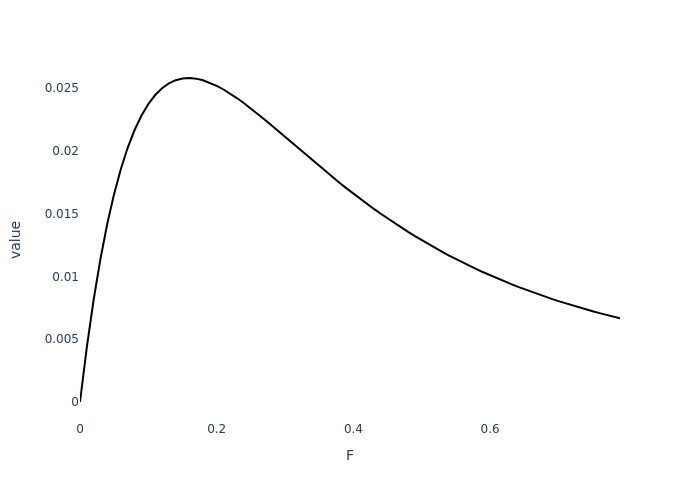
\includegraphics[width=\linewidth]{notebooks/SimpleOptimization/value_v_F.png}
  \caption{Value versus Fishing Mortality}
  \label{fig:value_v_F}
\end{figure}

And if we walk through this example we can see why optimization is so important. Start at $F=0$ we get an obvious result - if you don't fish you don't derive any value from the fishery. Then as we begin to apply some fishing pressure $F>0$ we can see that the value starts rising rapidly - also expected. However something really interesting happens once we cross $F\approx 0.2$ the value starts to go down! What's going on here? Well it turns out that after a certain point ramping up the fishing pressure starts to kill so many \textit{young} fish that fish aren't able to grow up to the big weights that are more valuable to the fishery. As a result the fishery actually becomes poorer as we put more effort in! More work does not mean more rewards because that extra work actually changes the very demographics of the underlying stock. Super interesting! 
\newline

Alright, so as we said this was a pretty simple example. Part of what made it so simple was our "management" was parametrized by a single variable $F$. This meant that we could just plot out all of the options and choose the best one. In theory this brute force approach can always work. While as you get to parametrizations that have more 3 parameters you lose the ability to plot things out you can still run through all of the options and pick the best one. However there's a practical problem that quickly arises and its known as the curse of dimensionality. 
\newline

To illustrate suppose you start with a single parameter case like ours, but one where the parameter is categorical (i.e. it takes on a specific set of values). Maybe that parameter can take on 10 values. This in turn means you need only search $10$ different cases to find your optimal case for sure. 
\newline

Alright, now suppose that you add another 10 value parameter. How many options do you have to search? Well for each of the original 10 values of our first parameter we need to search the other 10 from this new parameter. So that's $10\bullet 10=100$ different cases. If we add another parameter it becomes $10\bullet 10\bullet 10=1000$ values. You can probably see where this is going... in general $N$ such parameters means $10^N$ cases!
\newline

This gets computationally inefficient really really fast. So when folks optimize really large problems (with loads of parameters) they instead have to turn to things besides brute force search.
\newline

Generally speaking there are two categories - analytic and meta-heuristic. While going into either case would take up far too much room here the basic idea behind each is to use knowledge about the solutions you've already got to be clever about the next case you choose so you can quickly find better values without having to search the \textit{whole} space. But this doesn't come for free as most optimization algorithms can't guarantee optimality. Instead you have to carefully understand their drawbacks and gotchas so that you can make it highly probably that a global maximum (or something very close to it) will be found. The point - know your optimizer! 
\newpage

\noindent \rule{\textwidth}{0.5pt} 
\begin{figure}[h!] 
  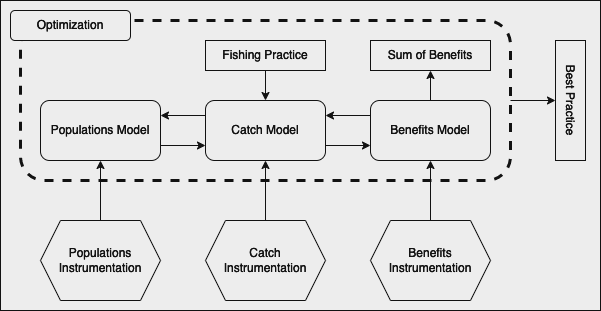
\includegraphics[width=\linewidth]{drawings/high_level.png}
  \caption{30,000ft View}
  \label{fig:high_level}
\end{figure}
\newline
\rule{\textwidth}{0.5pt} 
\vspace{5pt}

Hopefully at this point it's at least somewhat clear how this big problem breaks up into individual pieces. We've got models that drive our optimization, instrumentation creating ground truth data used to fit those models, and then the optimization itself. Put these together and you can find the right set of fishing parameters to maximize the long term value of the fishery. 
\newline

However it should also be clear how all of this is \textit{entirely} dependent on the models used and the fishing parameters chosen. So the question becomes - what can go wrong with the modeling itself? We turn to that next. 


\newpage

\bibliographystyle{plain}
\bibliography{reference}
\end{document}